\mySection{The Design of PyRollCall}
In this section, we present the use cases and the design of PyRollCall's architecture.
In the following context, a "user" refers to a "teacher" who wishes to perform roll calls
using PyRollCall, since the end user of this system is typically a teacher. In other words,
students are not the direct users of this system.
Figure~\ref{fig:use-case-diagram} shows the use case diagram of PyRollCall, whereas
Figure~\ref{fig:system-architecture} shows the system architecture of PyRollCall.


\subsection{Use Cases}
\vspace{0.3cm}

\setstretch{1.0}
\begin{itemize}
  \item Users can maintain the data of the courses and students they teach.
  \item Users can collect students' photos and generate their facial measurements.
  \item Users can start a roll call, recording students' attendace via FRT.
  \item Users can export the results of roll calls to files.
  \item Users should be able to keep their data the next time they use the system.
  \end{itemize}
\setstretch{\myContentLineSpacing}

\begin{figure}[!htb]
  \centering
  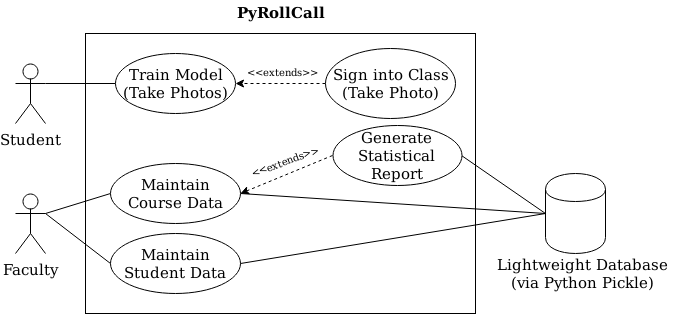
\includegraphics[width=\linewidth]{figures/use-case-diagram.png}
  \caption{Use Case Diagram}
  \label{fig:use-case-diagram}
\end{figure}

\begin{figure}[!htb]
  \centering
  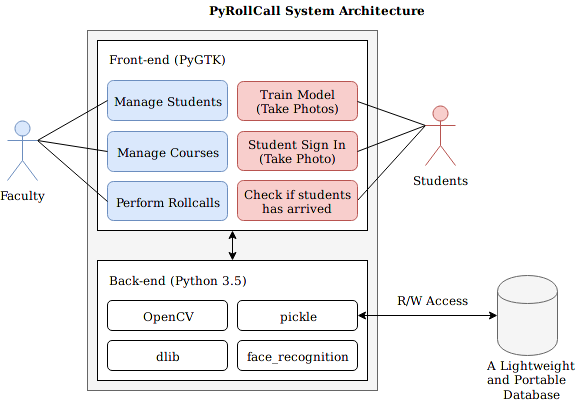
\includegraphics[width=\linewidth]{figures/system-architecture.png}
  \caption{System Architecture}
  \label{fig:system-architecture}
\end{figure}


\subsection{System Architecture}
Figure~\ref{fig:system-architecture} shows the system architecture of PyRollCall.
The GUI is built with \emph{PyGTK}, and it is already included in the project's \emph{virtualenv}, making
PyRollCall a highly portable system. The user can manage the data of courses and students,
take photos for students, compute their facial embeddings and perform roll calls via GUI\@.
Underneath the GUI, we use \emph{OpenCV} to capture images via cameras, \emph{face\_recognition} and \emph{dlib} to
recognize faces of students, and \emph{pickle}\footnote{pickle is a Python module
  which implements binary protocols to serialize and deserialize Python objects.}
to serialize and deserialize facial measurements (or facial embeddings).
\vspace{0.5cm}

The layout of project's root directory is presented in listing~\ref{lst:proj-root-layout}.
Note that trivial entries are omitted here for obvious reasons.
The entry point to the entire system is \emph{pyrollcoll.py}, whereas all modules are placed
inside the \emph{pyrollcall} directory. The user's data is stored in \emph{rollcall.db},
a lightweight database implemented with Python's pickle, inclusive of the courses he or she
teaches, the course-student mappings and all the pre-computed facial embeddings of students.
\vspace{0.2cm}

\begin{lstlisting}[numbers=none,xleftmargin=0em,caption={Layout of PyRollCall's root directory.},label={lst:proj-root-layout}]
$ ls -la
total 48K
drwxr-xr-x 3 aesophor aesophor 4.0K Dec  1 14:04 faces
drwxr-xr-x 2 aesophor aesophor 4.0K Jan 25 11:10 pyrollcall
drwxr-xr-x 5 aesophor aesophor 4.0K Nov 13 09:13 venv
drwxr-xr-x 7 aesophor aesophor 4.0K Jan 25 12:12 .git
-rw-r--r-- 1 aesophor aesophor  258 Jan 23 12:40 rollcall.db
-rwxr-xr-x 1 aesophor aesophor  197 Sep 26 20:33 pyrollcall.py
\end{lstlisting}
\vspace{0.2cm}

The \emph{pyrollcall} directory contains PyRollCall's modules and class definitions,
as shown in listing~\ref{lst:modules-and-classes}. Note that trivial entries are also
omitted here. Readers have probably noticed that there's also another \emph{pyrollcall.py}
in this directory, this module contains code that will initialize the user's data
from \emph{rollcall.db} and start the GUI, while the top-level \emph{pyrollcall.py} merely serves as the entry point to the system.

\begin{lstlisting}[numbers=none,xleftmargin=0em,caption={PyRollCall's modules and classes.},label={lst:modules-and-classes}]
$ ls -la pyrollcall
total 64K
-rw-r--r-- 1 aesophor aesophor 1.2K Sep 26 20:33 course.py
-rw-r--r-- 1 aesophor aesophor 3.1K Sep 26 20:33 database.py
-rw-r--r-- 1 aesophor aesophor 5.8K Jan 18 14:22 face.py
-rw-r--r-- 1 aesophor aesophor  493 Sep 26 20:33 __init__.py
-rw-r--r-- 1 aesophor aesophor  18K Sep 26 20:33 mainwindow.py
-rw-r--r-- 1 aesophor aesophor  399 Sep 26 20:33 pyrollcall.py
-rw-r--r-- 1 aesophor aesophor 2.0K Sep 26 20:33 session.py
-rw-r--r-- 1 aesophor aesophor  827 Sep 26 20:33 student.py
-rw-r--r-- 1 aesophor aesophor  399 Sep 26 20:33 utils.py
-rw-r--r-- 1 aesophor aesophor 4.2K Sep 26 20:33 widget.py
\end{lstlisting}
\vspace{0.2cm}

Among all modules, the most important one is \emph{face.py}, a module which contains code
to capture images with a camera, compute facial embeddings and recognize faces,
the details of which will be covered in the next subsection. The photos of
students should be of png format with their filename being \emph{name\_number.png}.
Furthermore, photos of a specific student should be grouped into a single directory
with the directory name being \emph{studentID\_name}. All directories containing students' photos
should be put in the \emph{faces} directory.
A minimal example is provided in listing~\ref{lst:faces-tree-output};
the student's name is "Marco" and the student's ID is "U10516045".
\vspace{0.2cm}

\begin{lstlisting}[numbers=none,xleftmargin=0em,caption={Example hierarchy of the \emph{faces} directory.},label={lst:faces-tree-output}]
$ tree faces 
faces
|___ U10516045_Marco
    |__ Marco_0.png
    |__ Marco_1.png

    1 directory, 2 files
\end{lstlisting}
\vspace{0.2cm}

To use PyRollCall completely without a camera connected to the computer,
simply follow the rules mentioned above and place the files in the corresponding directories
with correct filenames.

\subsection{Implementation}
The heart of PyRollCall is \emph{encode\_faces()} and \emph{recognize\_faces()} in \emph{face.py}.
The first function, encode\_faces(), enumerates all the images in the \emph{faces} directory
and compute the embeddings of each faces in the images. Each image in this directory
should contain exactly one face in order to prevent erroneous results during k-NN classification.

\emph{encode\_faces()} takes two arguments, an instance of Database and a string specifying
the absolute path to the \emph{faces} directory. It extracts the student's ID from the directory name,
get the bounding box of each face, compute the embeddings for faces inside the bounding boxes,
and save all the embeddings to the database. The idea is shown in Algorithm~\ref{alg:encode_faces}.
\vspace{0.2cm}

\begin{algorithm}
  \caption{Pre-compute facial embeddings (encodings) of all faces in the \emph{faces} directory.}
  \label{alg:encode_faces}
  \begin{algorithmic}
    \Procedure{encode\_faces}{database, faces\_dir}
    \For{\textbf{each} image \textbf{in} faces\_dir}
        \State $box \leftarrow get\_bounding\_box(image)$
        \State $e \leftarrow compute\_encoding(image, box)$
        \State $id \leftarrow get\_student\_id(image)$
        \State database.face\_encodings.insert(FaceEncoding(e, id)) 
      \EndFor
    \EndProcedure
  \end{algorithmic}
\end{algorithm}
\vspace{0.5cm}


\emph{recognize\_faces()} takes two arguments, an instance of Database and an image object.
Firstly, we detect all bounding boxes of the faces in the given image, and then
compute all facial encodings according to where these bounding boxes are located.
Secondly, for each facial encoding, we compare it with all known encodings from the database.
Each comparison should give us an array of boolean values, we can then count the votes
, find out which student has the highest vote, and mark that student as arrived.
The pseudo code is shown in Algorithm~\ref{alg:recognize_faces}.
\vspace{0.2cm}

\begin{algorithm}
  \caption{recognize\_faces(database, image)}
  \label{alg:recognize_faces}
  \begin{algorithmic}
    \Procedure{recognize\_faces}{database, image}
      \State $boxes \leftarrow get\_bounding\_boxes(image)$
      \State $encodings \leftarrow compute\_encodings(image, boxes)$
      \State 
      \For{\textbf{each} e $\in$ encodings}
        \State $votes \leftarrow compare\_faces(database.face\_encodings, e)$
        \State  $student \leftarrow get\_student\_with\_most\_votes(votes)$
        \State student.mark\_as\_arrived()
      \EndFor
    \EndProcedure
  \end{algorithmic}
\end{algorithm}
\vspace{0.5cm}

Please note that the pseudocode shown above differs from the actual implementation,
but the general idea are exactly the same.
